% ==============================================================================
% SECCION 3: ACTIVIDAD 2 - COMPARTICION DE CARGA (CHARGE SHARING) EN NAND3
% ==============================================================================
\clearpage
\section{Actividad 2: Compartición de Carga (Charge Sharing) en NAND3 Dinámica}
\label{sec:actividad2}

\subsection{Fundamento Físico y Predicción Analítica Previa}
En una compuerta NAND3 dinámica \textit{footed} con inversor dominó de salida, la red de descenso serie (PDN) posee nodos intermedios con capacitancias parásitas de difusión: $n_1$ (entre $M_1$ y $M_2$) y $n_2$ (entre $M_2$ y $M_3$). Tras un ciclo previo donde todos los nodos descargaron a $0\,\text{V}$ ($A=B=C=1$), si en la evaluación subsiguiente la compuerta conmuta a una condición donde la PDN permanece bloqueada a tierra pero los transistores superiores entran en conducción ($A=B=1, C=0$ con $CLK=1$):
\begin{enumerate}[leftmargin=1.4em,itemsep=0.15em]
  \item El transistor de precarga $M_p$ se apaga, dejando al nodo dinámico $dyn$ \textbf{flotante} cargado a $V_{DD} = 1.0\,\text{V}$.
  \item $M_3$ permanece en corte ($C=0$), manteniendo abierto el camino conductivo hacia el footer $M_f$ y tierra.
  \item $M_1$ y $M_2$ conducen ($A=B=1$), conectando el nodo $dyn$ con las capacitancias parásitas descargadas de $n_1$ y $n_2$.
  \item La carga electrostática almacenada en $C_{dyn}$ se redistribuye hacia $C_{n1}$ y $C_{n2}$, provocando una caída transitoria de potencial $\Delta V$ (\textit{charge sharing droop}).
\end{enumerate}

\noindent\textbf{Deducción de Capacitancias de Difusión ($C_a$):} Conforme a las geometrías de la guía ($L_{\text{diff}} = 90\,\text{nm}$, $W_{\text{PDN}} = 270\,\text{nm}$), el área de difusión es $Ad = W \times L_{\text{diff}} = 0.0243\,\mu\text{m}^2$ y el perímetro exterior $Pd = W + 2L_{\text{diff}} = 0.450\,\mu\text{m}$. Empleando los parámetros de unión de \texttt{ptm45hp.lib} ($c_j = 0.50\,\text{fF}/\mu\text{m}^2$, $c_{jsw} = 0.50\,\text{fF}/\mu\text{m}$), la capacitancia por contacto de difusión a cero sesgo resulta:
\begin{equation}
  C_{\text{diff},1} = c_j \cdot Ad + c_{jsw} \cdot Pd = 0.01215\,\text{fF} + 0.22500\,\text{fF} = 0.23715\,\text{fF}
\end{equation}
donde el efecto tridimensional perimetral (\textit{sidewall}) concentra el $94.9\%$ de la capacidad total. Dado que cada nodo interno $n_1$ y $n_2$ comparte dos difusiones adyacentes ($C_{n1} = C_{n2} = 2\,C_{\text{diff},1} = 0.4743\,\text{fF}$), la capacitancia agregada descargada es:
\begin{equation}
  C_a \equiv C_{n1} + C_{n2} = 0.9486\,\text{fF}
\end{equation}

\noindent\textbf{Modelo Analítico Ideal de Conservación de Carga:} Asumiendo transistores ideales como conmutadores perfectos sin caída de umbral, el reparto puro de carga predice:
\begin{equation}
  Q_{\text{inicial}} = C_{dyn} V_{DD} = (C_{dyn} + C_a) V_{dyn,\text{final}} \implies \Delta V_{\text{pred}} = V_{DD} \cdot \frac{C_a}{C_a + C_{dyn}}
  \label{eq:charge_sharing}
\end{equation}
Para la condición nominal ($C_L = 2.0\,\text{fF}$) y considerando las parásitas fijas en $dyn$ según la guía ($C_{\text{extra}} = C_{gd}(M_p) + C_g(\text{inversor}) \approx 0.3441\,\text{fF} \implies C_{dyn} \approx 2.3441\,\text{fF}$), la caída teórica predicha es:
\begin{equation}
  \Delta V_{\text{pred}} = 1.0\,\text{V} \cdot \frac{0.9486\,\text{fF}}{0.9486\,\text{fF} + 2.3441\,\text{fF}} = \mathbf{288.09\,\text{mV}} \implies V_{dyn,\text{pred}} = 0.7119\,\text{V}
\end{equation}
\textit{Nota metodológica:} Esta formulación de primer orden es idealizada: omite componentes del modelo BSIM4 (como la capacitancia de borde compuerta-difusión $c_{jswgs}$) y no contempla la dinámica de conducción no lineal ni el corte progresivo del stack.

\subsection{Estímulo Literal de la Guía vs Benchmark Físico Controlado}
Con el estímulo literal de la guía oficial, el instante temporal especificado ($t = 1.95\,T_{clk} = 3.9\,\text{ns}$) coincide con la fase de precarga para la temporización empleada a $500\,\text{MHz}$ ($CLK=0$), provocando que la conducción activa de $M_p$ recargue continuamente el nodo dinámico y enmascare la redistribución hacia los nodos internos. Por ello, se conservó dicha corrida oficial de referencia y se implementó un ensayo de benchmark físico controlado (\texttt{ENS-A2-02}) que garantiza:
\begin{enumerate}[leftmargin=1.4em,itemsep=0.15em]
  \item Descarga completa previa de $dyn, n_1, n_2, n_3$ a $0\,\text{V}$ durante un primer ciclo de evaluación ($A=B=C=1$).
  \item Precarga exclusiva de $dyn$ a $V_{DD}$ en el semi-periodo bajo subsiguiente ($CLK=0$), manteniendo $n_1$ y $n_2$ descargados.
  \item Entrada en evaluación ($CLK=1, M_p$ en corte) con transición $A=B=1, C=0$, aislando con total fidelidad el fenómeno de \textit{charge sharing}.
\end{enumerate}

\begin{figure}[htbp]
  \centering
  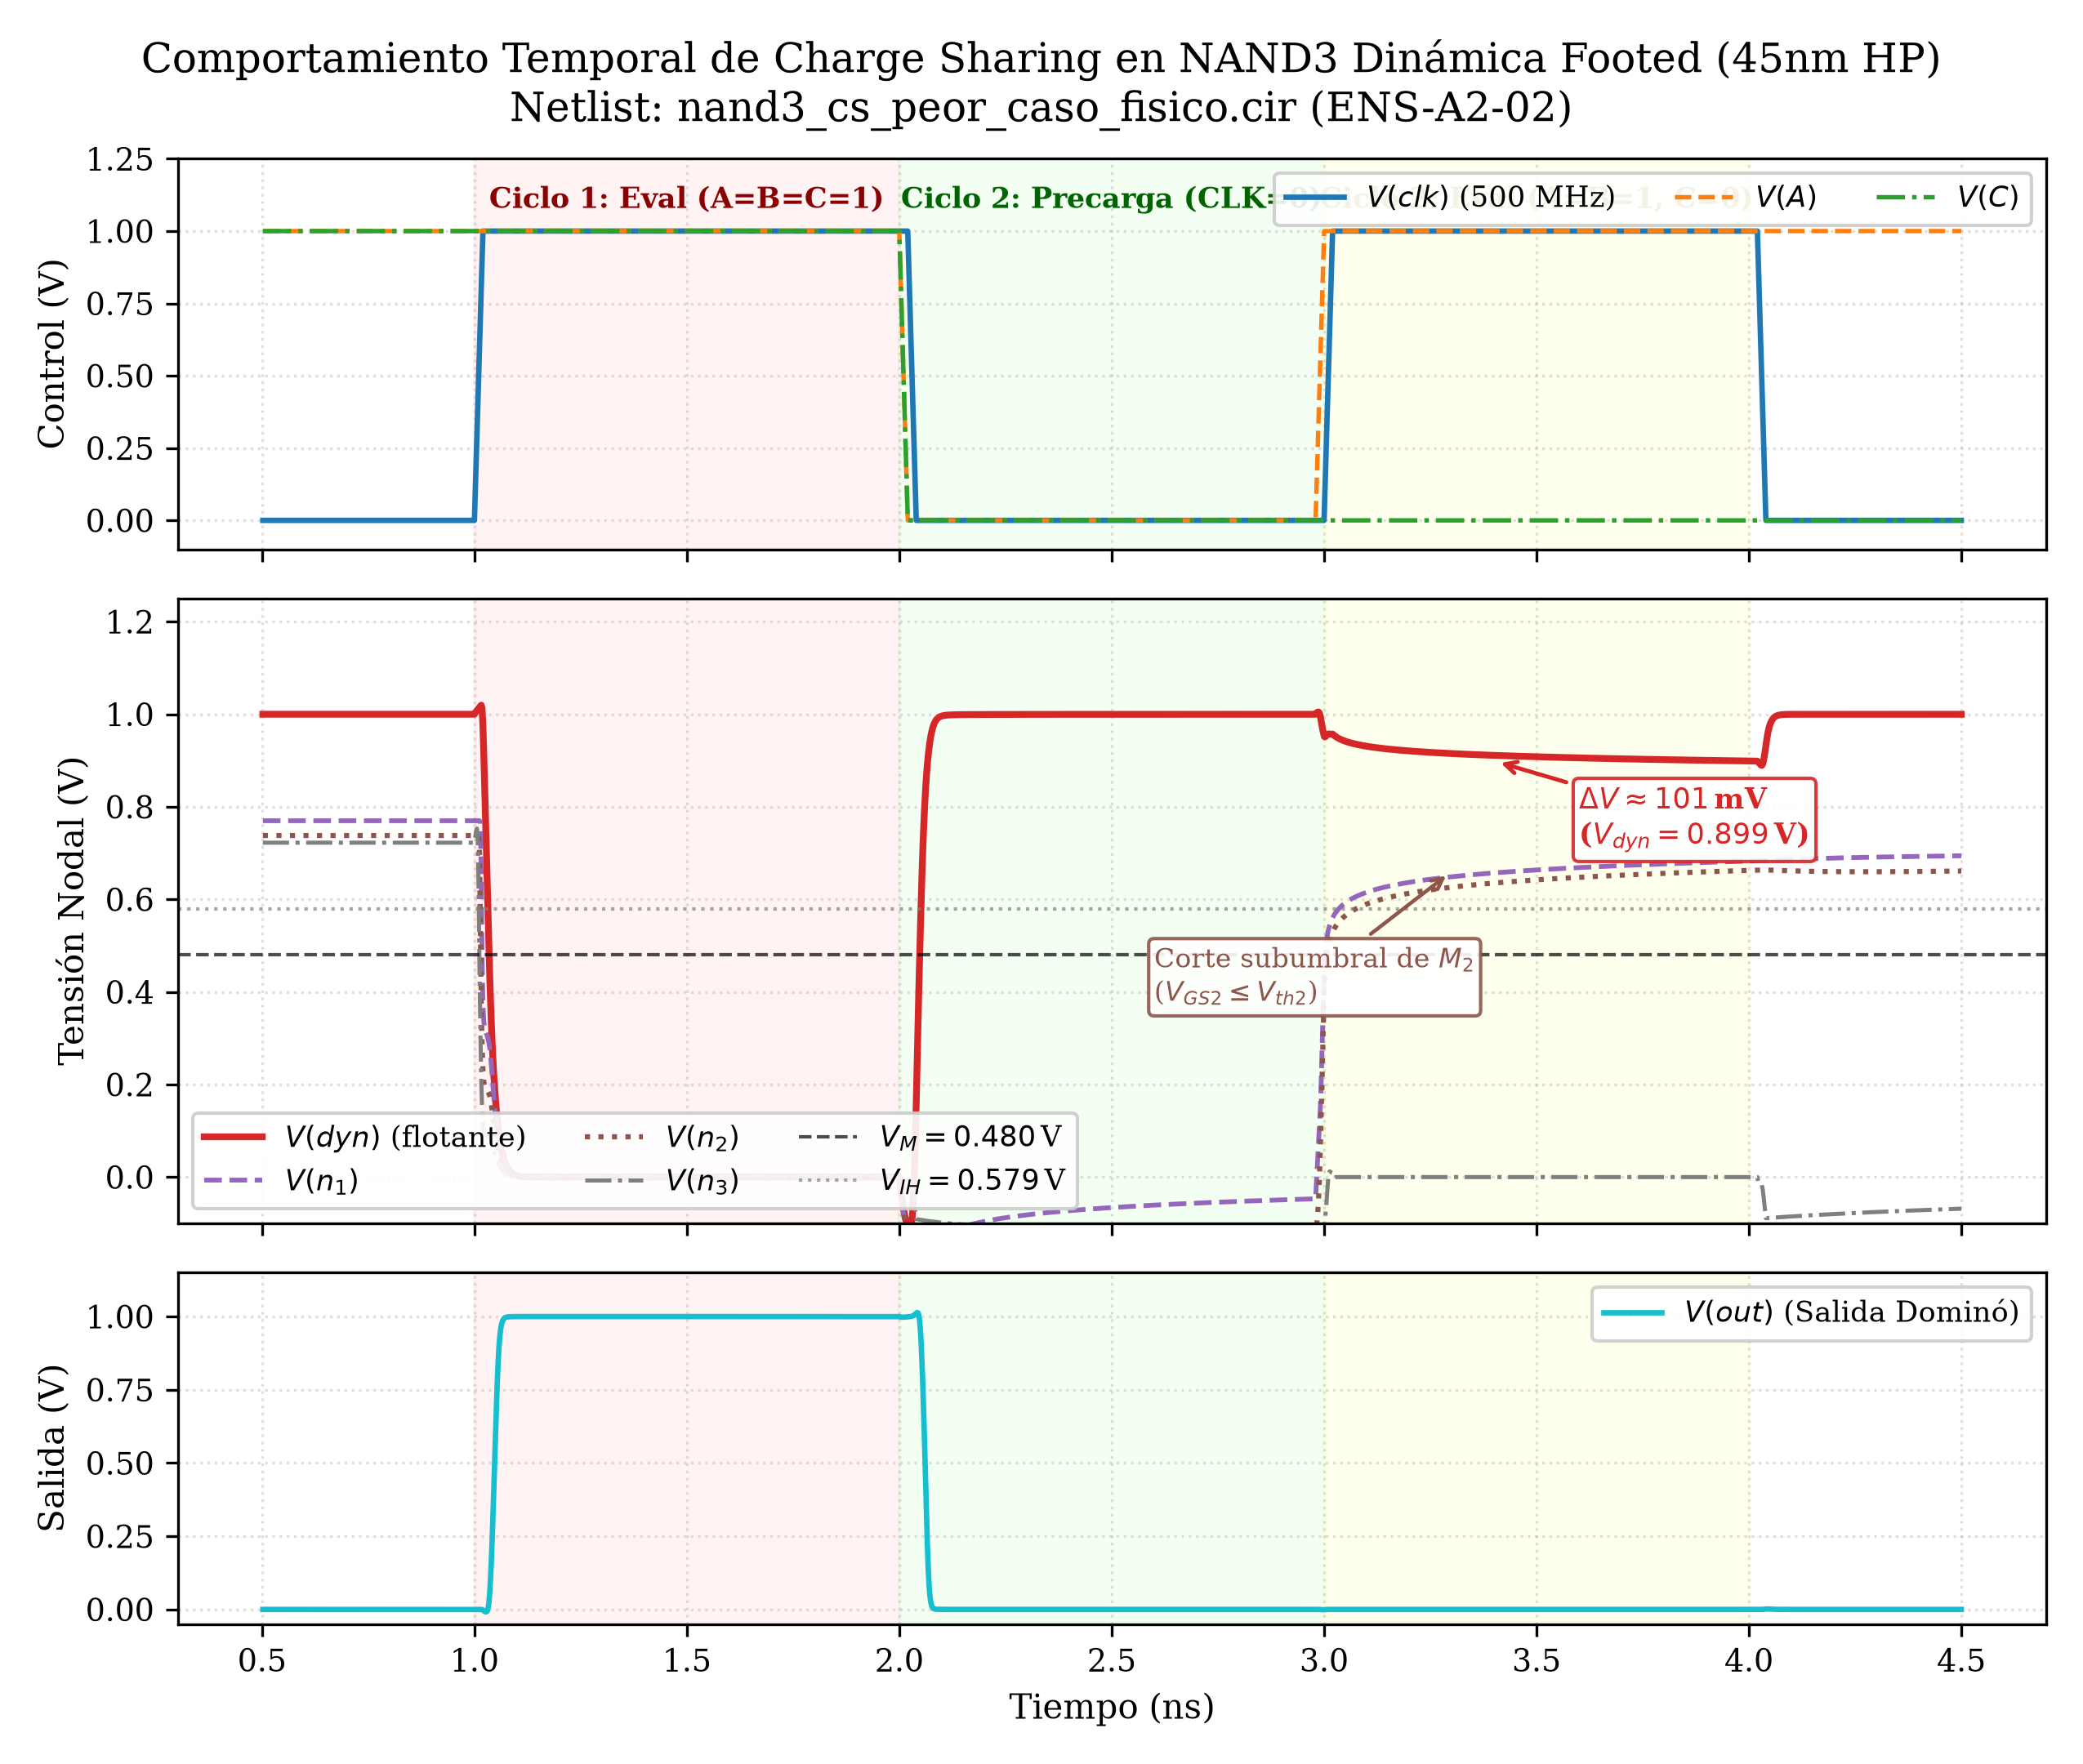
\includegraphics[width=0.68\linewidth]{figuras/fig1_act2_peor_caso_formas_onda.png}
  \caption[Formas de onda sincronizadas del peor caso de charge sharing]{Formas de onda sincronizadas del peor caso de charge sharing en la NAND3 dinámica footed (control $CLK, A, C$, nodos internos $n_1, n_2, n_3$, nodo $dyn$ y salida $out$).}
  \label{fig:peor_caso_formas_onda}
\end{figure}

\subsection{Resultados del Caso Base y Discrepancia Física}
La simulación del caso base nominal ($C_L = 2.0\,\text{fF}$, Figura~\ref{fig:peor_caso_formas_onda}) registra una caída de $\Delta V_{\text{sim}} = \mathbf{101.03\,\text{mV}}$, alcanzando un mínimo de $V_{dyn,\text{min}} = \mathbf{0.8990\,\text{V}}$, sin inducir conmutación espuria en la salida dominó ($V_{out,\text{max}} = 0.149\,\text{mV} \ll V_{IL} = 0.3675\,\text{V}$). 

La caída simulada es $2.85\times$ menor a la predicción teórica ($\Delta V_{\text{pred}} = 288.09\,\text{mV}$). Esta discrepancia no obedece a un error de cálculo, sino a la física intrínseca del transistor MOS:
\begin{enumerate}[leftmargin=1.4em,itemsep=0.15em]
  \item \textbf{Corte Subumbral del Transistor Pasante ($M_2$):} $M_2$ opera como transistor de paso con compuerta en $V_B = 1.0\,\text{V}$. Al transferirse carga hacia $n_2$, la tensión $V(n_2)$ se eleva. Debido a que el sustrato está polarizado a masa ($0\,\text{V}$), se desarrolla un efecto de cuerpo severo ($V_{SB2} = V(n_2) > 0$). Evaluando analíticamente la elevación de umbral mediante la formulación clásica $\Delta V_{th} \approx k_1 (\sqrt{2\phi_F + V_{SB}} - \sqrt{2\phi_F})$ con los parámetros de la tarjeta PTM ($k_1 = 0.4\,\text{V}^{1/2}$, $2\phi_F \approx 0.8\,\text{V}$), se obtiene una \textbf{estimación analítica aproximada} de $V_{th,\text{eff}} \approx 0.55\text{ a } 0.60\,\text{V}$ (frente a $V_{th0} = 0.469\,\text{V}$ a cero sesgo). Al subir $V(n_2)$ hasta $\approx 0.66\,\text{V}$, la tensión compuerta-fuente cae a $V_{GS2} = 1.0 - 0.66 = 0.34\,\text{V} \ll V_{th,\text{eff}}$, forzando a $M_2$ a entrar en régimen subumbral y bloqueando el flujo de carga antes de alcanzar el equilibrio estático total.
  \item \textbf{No Linealidad de Capacitancias de Unión:} Conforme $n_1$ y $n_2$ aumentan su tensión respecto a masa, la polarización inversa de las uniones $p\text{-}n$ reduce dinámicamente la capacitancia neta según $C_j(V_R) = C_{j0} / (1 + V_R/PB)^M$.
\end{enumerate}

\subsection{Barrido Paramétrico de Carga (\texorpdfstring{$C_L$}{CL}) y Márgenes de Ruido}
Se simuló el comportamiento ante variaciones de $C_L \in [0.5,\, 1.0,\, 2.0,\, 4.0]\,\text{fF}$. Los resultados cuantitativos contrastados con el modelo analítico se presentan en la Tabla~\ref{tab:barrido_cl_act2}, y su comportamiento gráfico en la Figura~\ref{fig:dv_vs_cl}.

% Tabla de barrido parametrico de capacitancia de carga en Actividad 2
% Fuentes de datos: act2_metricas.json (g2b_sincrono_barrido_cl + series historicas)
\begin{table}[htbp]
\centering
\scriptsize
\caption[Barrido paramétrico de capacitancia de carga y caída por redistribución]{Barrido paramétrico de la capacitancia de carga $C_L$ en el nodo dinámico: contraste entre predicción analítica ($\Delta V_{\text{pred}}$), simulación del protocolo síncrono nominal ($\Delta V_{\text{sinc}}$) y protocolo alternativo con entradas anticipadas ($\Delta V_{\text{anticip}}$) bajo PTM 45\,nm HP ($V_{DD}=1.0\,\text{V}$).}
\label{tab:barrido_cl_act2}
\begin{tabularx}{\linewidth}{@{}>{\centering\arraybackslash}p{1.2cm} c c c c c >{\RaggedRight\arraybackslash}X@{}}
\toprule
\textbf{$C_L$} & \textbf{$\Delta V_{\text{pred}}$ (Guía)} & \textbf{$\Delta V_{\text{pred}}$ (Total)} & \textbf{$\Delta V_{\text{sinc}}$ (Nominal)} & \textbf{$V_{dyn,\text{min}}$ (Sinc)} & \textbf{$\Delta V_{\text{anticip}}$} & \textbf{Estado Lógico / Margen} \\
\textbf{(fF)} & \textbf{(mV)} & \textbf{(mV)} & \textbf{(mV)} & \textbf{(V)} & \textbf{(mV)} & \textbf{($V_{IH}=0.579\,\text{V}$, $V_M=0.480\,\text{V}$)} \\
\midrule
0.5 & 529.15 & 467.34 & \textbf{364.85} & 0.6351 & 175.92 & Seguro ($V_{dyn} > V_{IH} + 56\,\text{mV}$) \\
1.0 & 413.75 & 374.97 & \textbf{265.93} & 0.7341 & 138.26 & Seguro ($V_{dyn} > V_{IH} + 155\,\text{mV}$) \\
2.0 & 288.09 & 268.74 & \textbf{164.29} & 0.8357 & 101.03 & Seguro ($V_{dyn} > V_{IH} + 257\,\text{mV}$) \\
4.0 & 179.23 & 171.54 & \textbf{92.60}  & 0.9074 & 67.62  & Seguro ($V_{dyn} > V_{IH} + 328\,\text{mV}$) \\
\bottomrule
\end{tabularx}
\end{table}


\begin{figure}[htbp]
  \centering
  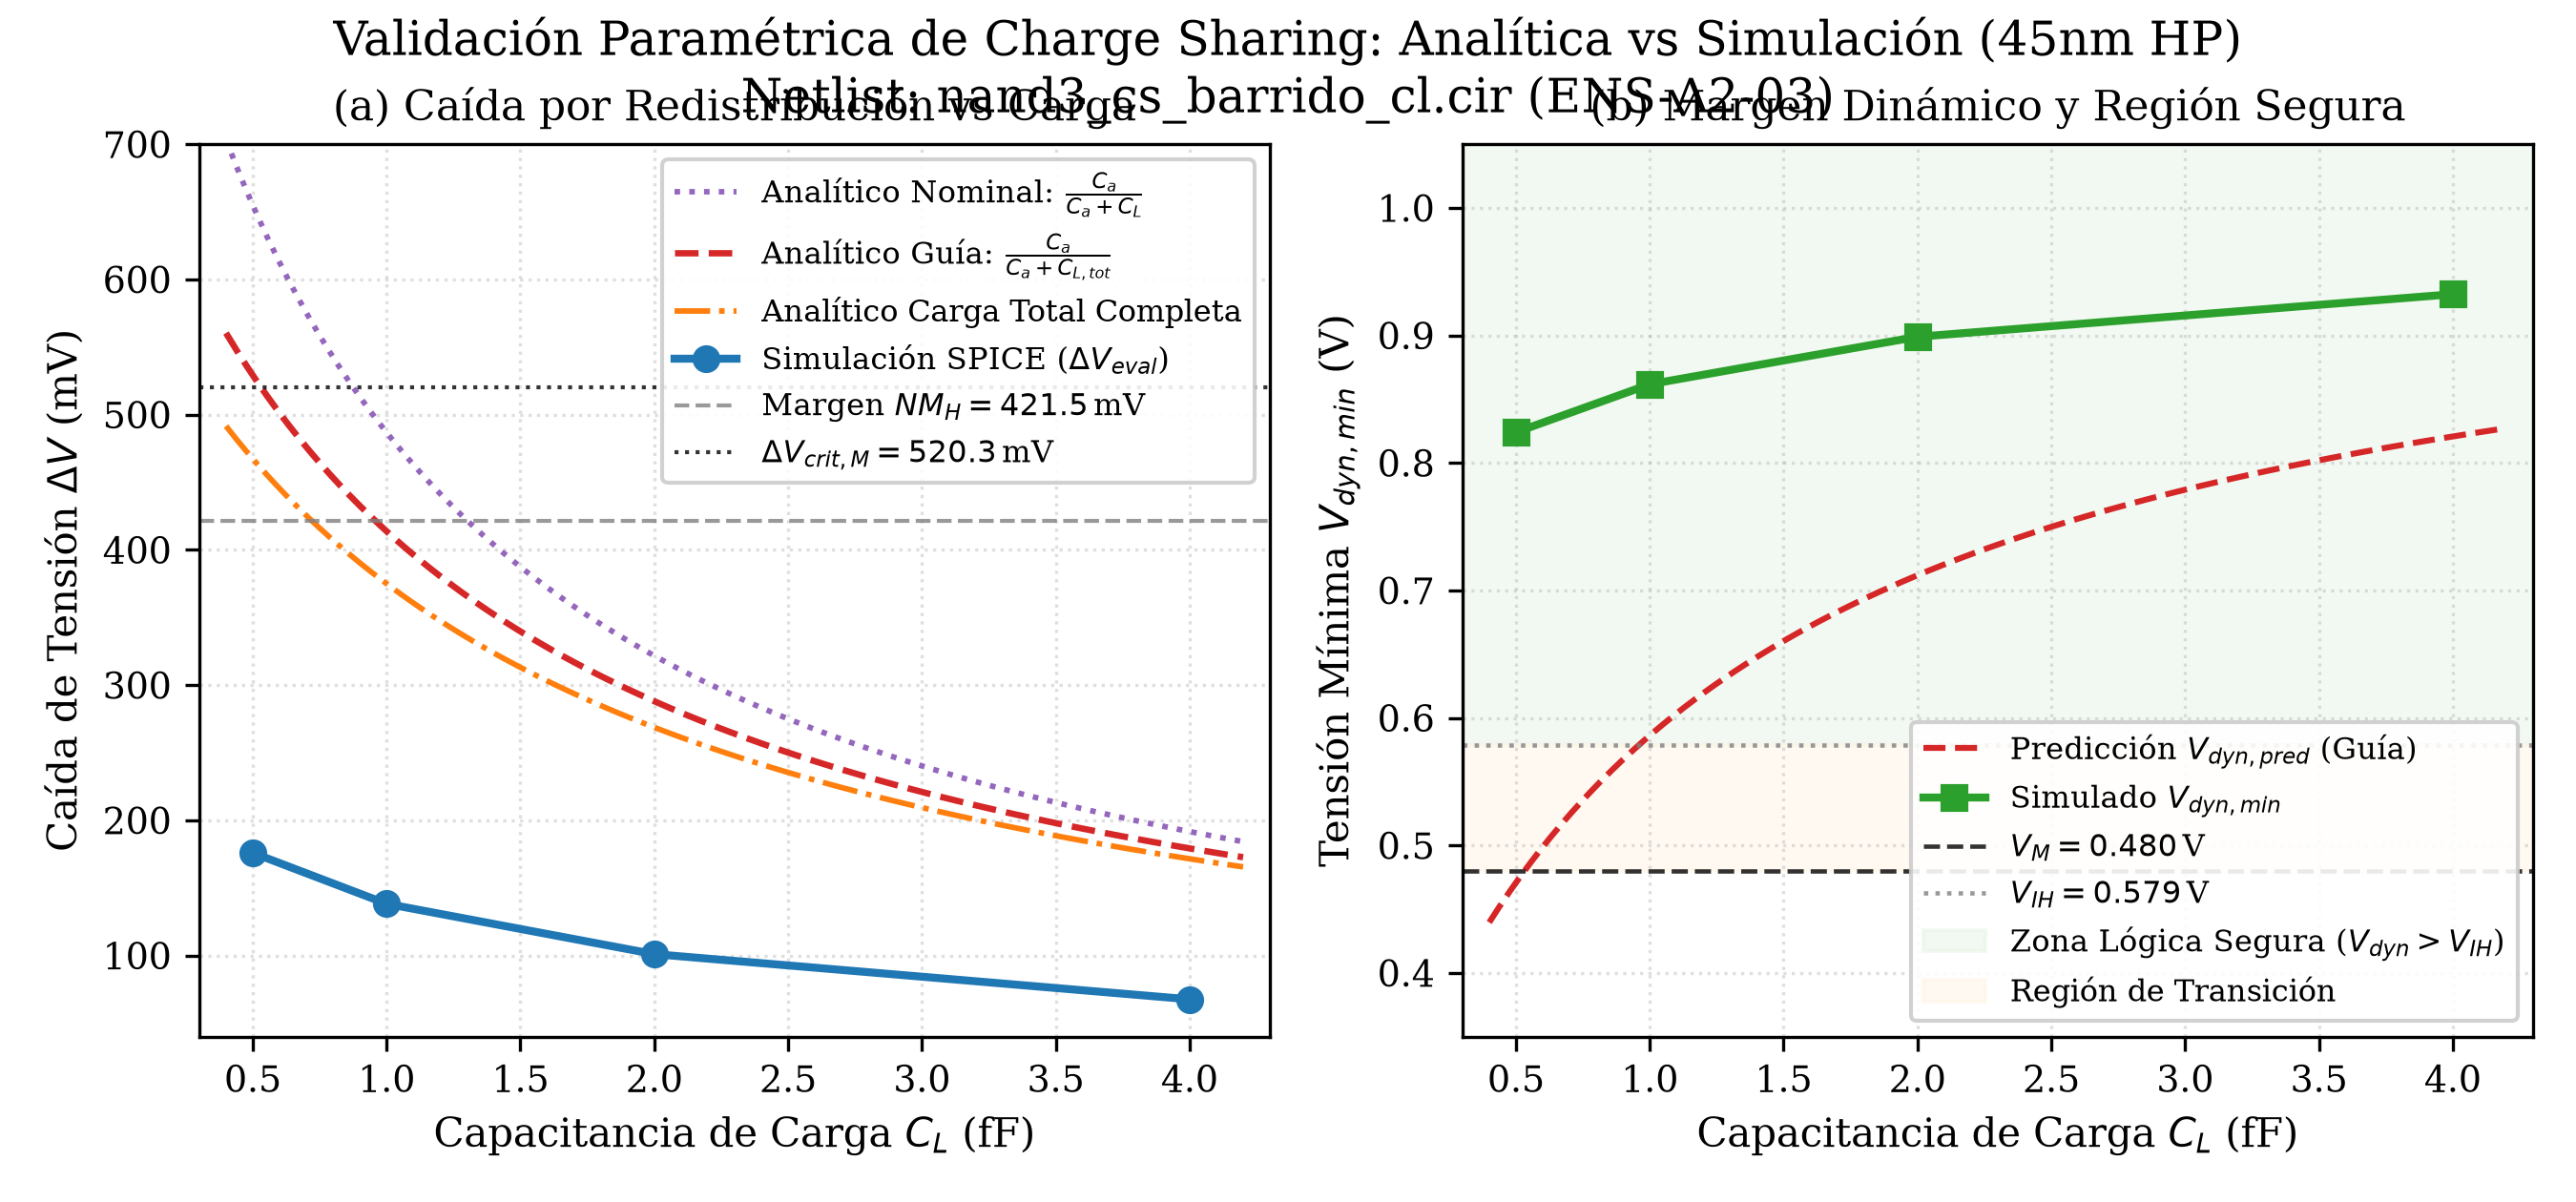
\includegraphics[width=0.68\linewidth]{figuras/fig2_act2_dv_vs_cl_analitico_simulado.png}
  \caption[Validación paramétrica de charge sharing vs capacitancia de carga]{Validación paramétrica de charge sharing frente a $C_L$: (a) Caída de potencial $\Delta V$ analítica vs simulación SPICE; (b) Tensión mínima $V_{dyn,\text{min}}$ y delimitación de la zona lógica segura frente a umbrales del inversor dominó ($V_M = 0.480\,\text{V}$, $V_{IH} = 0.579\,\text{V}$).}
  \label{fig:dv_vs_cl}
\end{figure}

\noindent\textbf{Tendencia Física e Inmunidad al Ruido:} A mayor capacitancia $C_L$, menor es la caída $\Delta V$ debido al incremento del depósito de carga inicial $Q = C_{dyn} V_{DD}$. En todos los casos ensayados, el nodo $dyn$ permanece rígidamente dentro de la zona lógica segura ($V_{dyn,\text{min}} \ge 0.8241\,\text{V} > V_{IH} = 0.5785\,\text{V}$), evitando falsas conmutaciones. Cabe resaltar que si la redistribución hubiese seguido el modelo lineal sin corte de umbral, para $C_L = 0.5\,\text{fF}$ la caída predicha ($\Delta V_{\text{pred}} = 529.15\,\text{mV}$) habría sumergido a $V(dyn)$ en $0.4708\,\text{V} < V_M$, generando un fallo lógico destructivo en la salida; el corte subumbral intrínseco del NMOS actúa así como una barrera protectora natural de integridad lógica.

\subsection{Evaluación Cuantitativa de Técnicas de Mitigación}
Bajo las condiciones de peor caso ($C_L = 2.0\,\text{fF}$), se implementaron y caracterizaron las tres técnicas de mitigación estipuladas en la guía. Los resultados comparativos se sintetizan en la Tabla~\ref{tab:mitigaciones_act2} y en la Figura~\ref{fig:comparacion_mitigaciones}.

% Tabla cuantitativa de tecnicas de mitigacion en Actividad 2
% Fuentes de datos: act2_metricas.json (g2b_sincrono_piloto_cl2f, g2b_sincrono_reordenamiento, g2c_precarga, g2c_keeper, g2c_contencion)
\begin{table}[htbp]
\centering
\fontsize{7pt}{8.3pt}\selectfont
\caption[Evaluación cuantitativa y trade-offs de técnicas de mitigación]{Evaluación cuantitativa de técnicas de mitigación de compartición de carga en NAND3 dinámica footed ($C_L=2.0\,\text{fF}$, $T_{clk}=2\,\text{ns}$, PTM 45\,nm HP, $V_{DD}=1.0\,\text{V}$). Márgenes referidos a $V_{IH}=0.5785\,\text{V}$ del inversor ($NM_H \equiv V_{dyn,\text{min}} - V_{IH}$) y áreas referidas a $W_{\text{dyn,base}} = 1215\,\text{nm}$ ($W_{\text{celda,base}} = 1440\,\text{nm}$).}
\label{tab:mitigaciones_act2}
\begin{tabularx}{\linewidth}{@{}>{\RaggedRight\arraybackslash}p{2.3cm} >{\centering\arraybackslash}p{1.6cm} >{\centering\arraybackslash}p{1.7cm} >{\centering\arraybackslash}p{1.7cm} >{\centering\arraybackslash}p{1.3cm} >{\RaggedRight\arraybackslash}X@{}}
\toprule
\textbf{Configuración} & \textbf{$\Delta V_{\text{eval}}$ / Extremo} & \textbf{Margen $NM_H$} & \textbf{Área Extra ($\Delta W$)} & \textbf{Carga $CLK$} & \textbf{Compromiso y Dinámica (Trade-off)} \\
\midrule
\textbf{Caso Base Síncrono} & \textbf{164.29\,mV} ($0.8357\,\text{V}$) & \textbf{+257.2\,mV} ($V_M+356\,\text{mV}$) & 0 ($0.0\%$) & Base ($0.50\,\text{fF}$) & Sin recuperación en evaluación ($V_{dyn,\text{end}} = 0.8357\,\text{V}$). Salida dominó inmune ($V_{out,\text{max}} \le 0.13\,\text{mV} \ll V_{IL}$). \\
\textbf{Precarga $W_p=45\,\text{nm}$} & \textbf{$-50.47$\,mV} ($1.0505\,\text{V}$) & \textbf{+472.0\,mV} & +2 PMOS ($90\,\text{nm}$, $+7.4\%$) & $+0.127\,\text{fF}$ ($63.7\,\text{nW}$) & Suprime droop; sobreimpulso capacitivo $+50.5\,\text{mV}$. Variante óptima en consumo de reloj. \\
\textbf{Precarga $W_p=135\,\text{nm}$} & \textbf{$-50.47$\,mV} ($1.0505\,\text{V}$) & \textbf{+472.0\,mV} & +2 PMOS ($270\,\text{nm}$, $+22.2\%$) & $+0.382\,\text{fF}$ ($191.1\,\text{nW}$) & Idéntica eficacia nominal que $45\,\text{nm}$, pero con $3.0\times$ sobrecoste capacitivo y de potencia en reloj. \\
\textbf{Reordenamiento C-B-A} & V.A: $\le 0$ / V.B: \textbf{164.3\,mV} & V.A: $+443.5$ / V.B: $+257.2$ & 0 transistores ($0.0\%$) & 0 fF en $CLK$ & Eficaz para Vect A ($C=0$ en tope bloquea $dyn$); vulnerable a Vect B ($A=0$ en base reproduce caída base). \\
\textbf{Reordenamiento C-A-B} & V.A: $\le 0$ / V.B: \textbf{72.08\,mV} & V.A: $+443.5$ / V.B: $+349.4$ & 0 transistores ($0.0\%$) & 0 fF en $CLK$ & Suprime Vect A y acota Vect B a $72.1\,\text{mV}$ (droop $-56.1\%$) al aislar $n_2$. Coste en complejidad de ruteo. \\
\textbf{Keeper $W_{kp}=45\,\text{nm}$} & \textbf{69.68\,mV} ($0.9303\,\text{V}$) & \textbf{+351.8\,mV} (mín.) & +1 PMOS ($45\,\text{nm}$, $+3.7\%$) & 0 fF en $CLK$ & Caída en $69.7\,\text{mV}$; restaura en $92.9\,\text{ps}$ y finaliza en $0.9996\,\text{V}$ ($99.96\%$). Contención: $+14.65\%$ en $t_{pHL,dyn}$. \\
\bottomrule
\end{tabularx}
\end{table}


\begin{figure}[htbp]
  \centering
  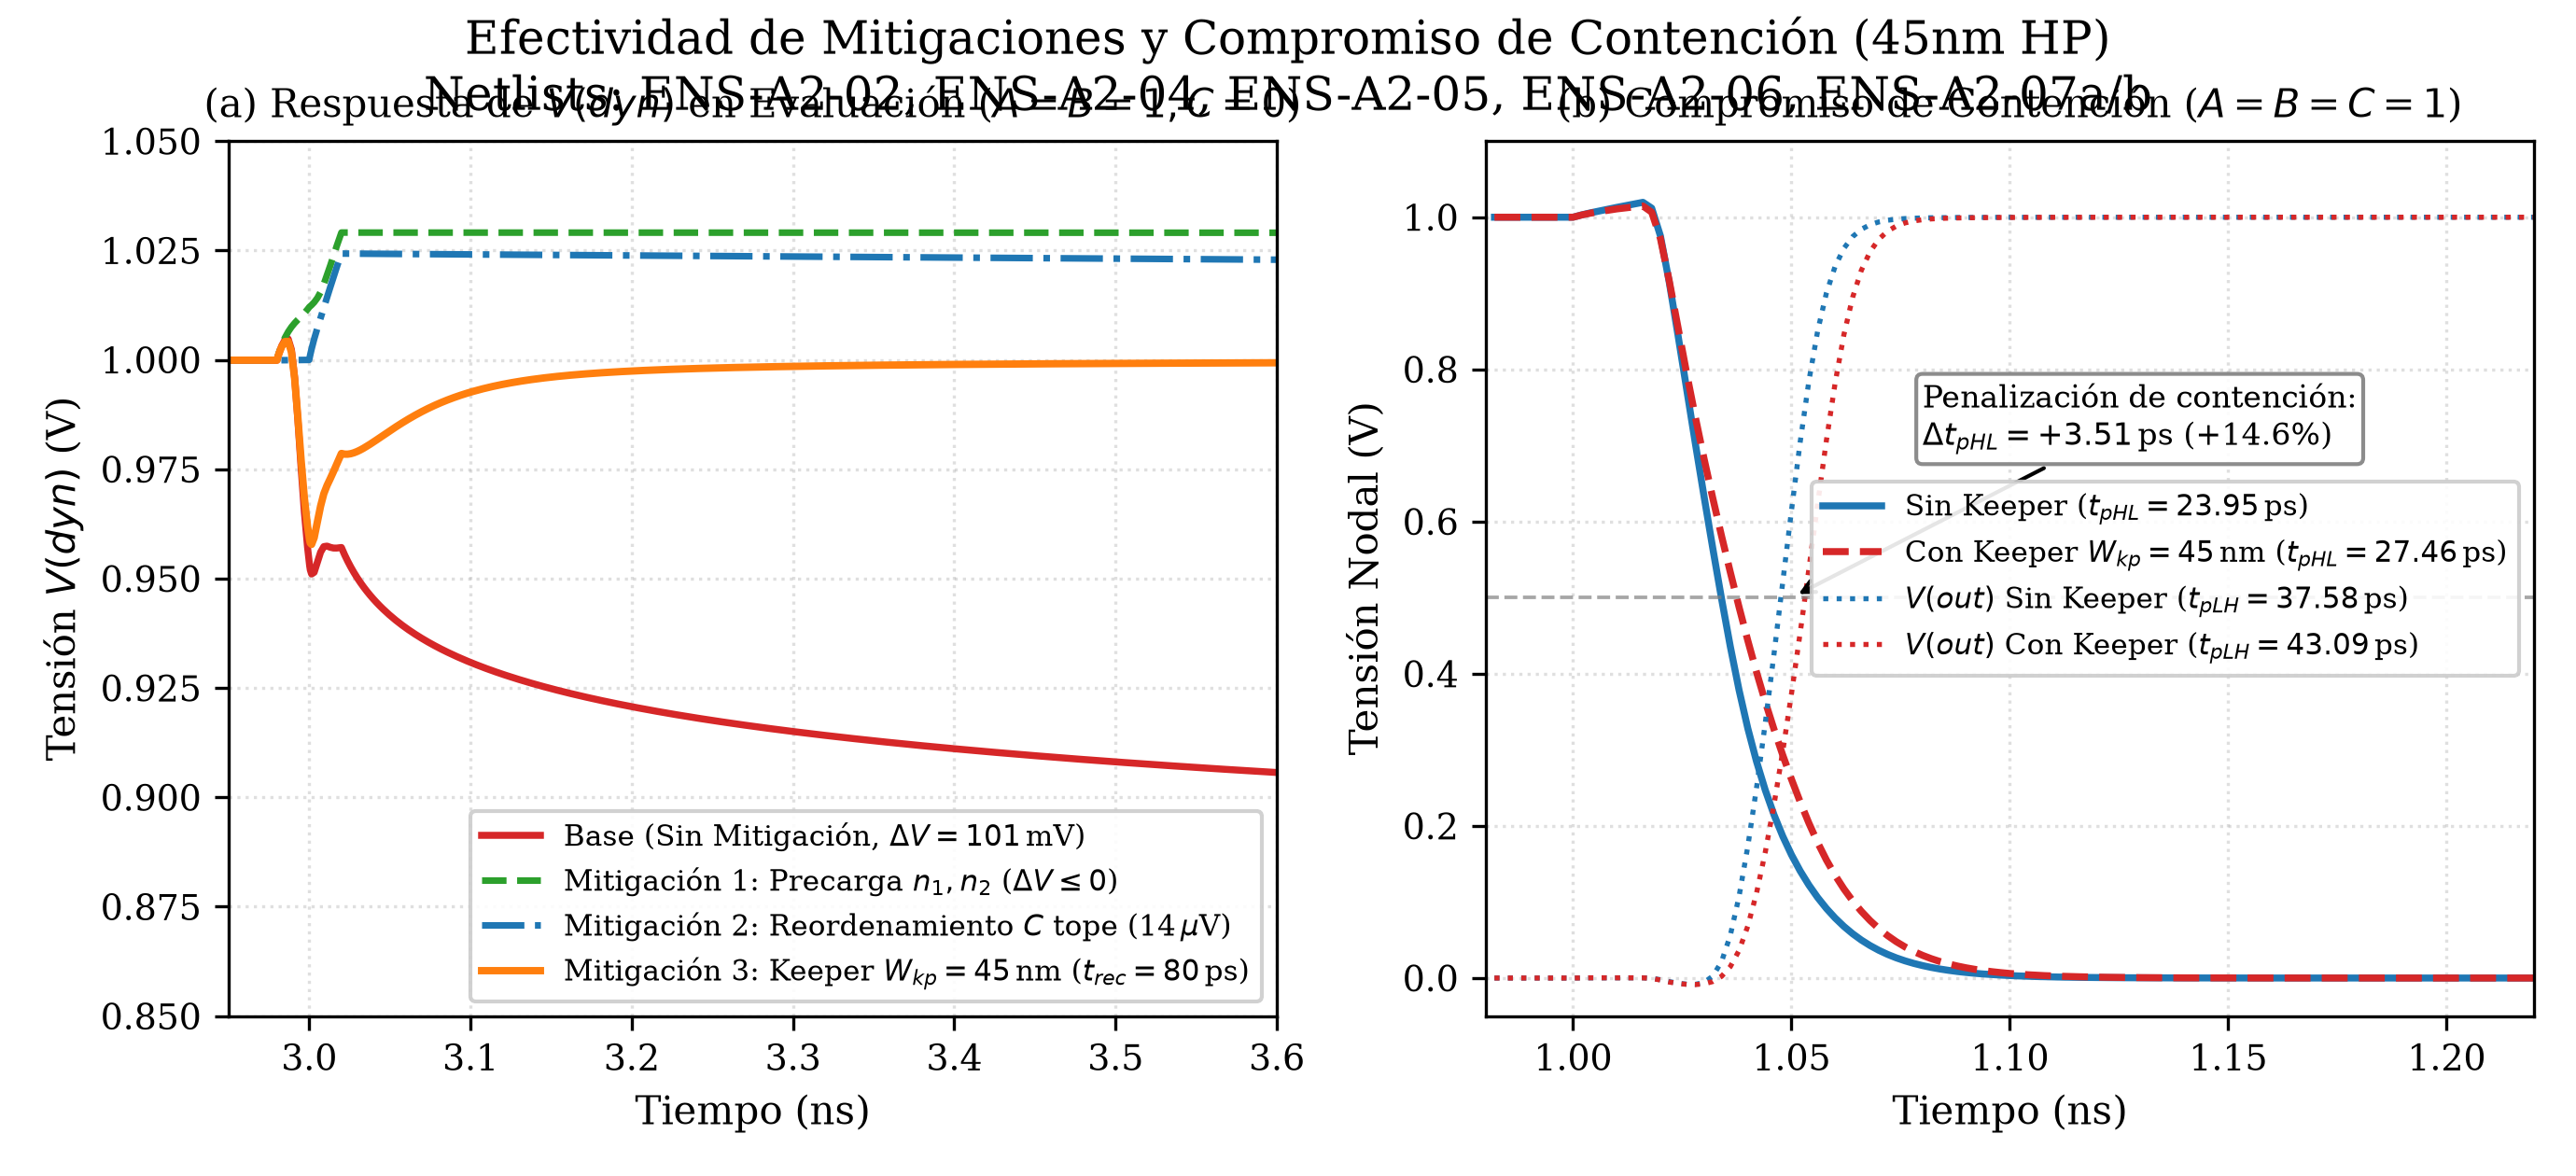
\includegraphics[width=0.68\linewidth]{figuras/fig3_act2_comparacion_mitigaciones.png}
  \caption[Comparación de técnicas de mitigación y compromiso de contención]{Comparación cuantitativa de técnicas de mitigación de charge sharing: (a) Formas de onda transitorias de $V(dyn)$ durante evaluación; (b) Compromiso de contención del keeper ($W_{kp}=45\,\text{nm}$) en retardo durante conmutación legítima ($A=B=C=1$).}
  \label{fig:comparacion_mitigaciones}
\end{figure}

\subsubsection{Técnica 1: Precarga de Nodos Internos (\texorpdfstring{$n_1, n_2$}{n1, n2})}
Se incorporaron dos transistores PMOS auxiliares ($W_p = 135\,\text{nm}$) comandados por $CLK$ para precargar los nodos internos $n_1$ y $n_2$ a $V_{DD}$ durante $CLK=0$. 
\begin{itemize}[leftmargin=1.4em,itemsep=0.15em]
  \item \textbf{Efectividad y Droop:} Al igualar las tensiones iniciales ($V(dyn) = V(n_1) = V(n_2) = V_{DD}$), la fuerza impulsora de redistribución se anula, suprimiendo completamente la caída ($\Delta V \le 0\,\text{mV}$).
  \item \textbf{Sobrecarga de Reloj:} La adición de dos compuertas PMOS introduce una capacitancia parásita adicional en la línea de reloj estimada en $\Delta C_{clk,\text{gate}} \approx 2(W_p \cdot L \cdot C_{ox}) \approx \mathbf{0.34\,\text{fF}}$, lo cual supone un incremento relativo de compuerta del $+67\%$ respecto a la carga de reloj base ($C_{g,Mp} + C_{g,Mf} \approx 0.503\,\text{fF}$).
  \item \textbf{Overshoot por Acoplamiento Transitorio:} Se aprecia un sobreimpulso nodal por acoplamiento capacitivo (\textit{clock feedthrough / bootstrap-like}): $V_{dyn,\text{min}} = 1.0120\,\text{V}$, $V(n_1) \approx 1.069\,\text{V}$ y $V(n_2) \approx 1.062\,\text{V}$. Si bien no induce conmutación espuria ($V_{out,\text{max}} \le 0.27\,\text{mV}$), debe considerarse en el diseño de márgenes de tensión.
  \item \textbf{¿Por qué no se precarga el nodo $n_3$?} El nodo $n_3$ conecta directamente al drenaje del footer $M_f$. Al entrar en evaluación ($CLK \to 1$), $M_f$ conduce inmediatamente hacia tierra. Precargar $n_3$ forzaría una descarga innecesaria a masa en cada ciclo de reloj, incurriendo en una disipación dinámica redundante $C_{n3} V_{DD}^2 f_{clk}$ sin beneficio alguno, dado que cuando $C=0$, $M_3$ permanece en corte y $n_3$ jamás interactúa con el nodo dinámico.
\end{itemize}

\subsubsection{Técnica 2: Reordenamiento de Entradas en la PDN}
Consiste en asignar la entrada crítica que permanece en nivel bajo ($C=0$) al transistor más próximo al nodo dinámico ($M_3$ adyacente a $dyn$), relegando las entradas en nivel alto ($A, B$) a las posiciones inferiores.
\begin{itemize}[leftmargin=1.4em,itemsep=0.15em]
  \item \textbf{Rendimiento:} Al encontrarse $M_3$ bloqueado en el propio contacto superior, las capacitancias parásitas de $n_1$ y $n_2$ quedan físicamente aisladas de $dyn$. La perturbación se reduce drásticamente a $\Delta V = \mathbf{14.1\,\mu\text{V}}$ ($V_{dyn} = 0.99999\,\text{V}$).
  \item \textbf{Coste:} No requiere transistores adicionales ($0$ PMOS) ni agrega carga a la línea de reloj ($0\,\text{fF}$). Su implementación involucra exclusivamente decisiones de enrutamiento y asignación de pines en layout.
  \item \textbf{Asimetría Lógica Dominó vs Lógica Estática:} En lógica CMOS estática, el orden de apilamiento en la PDN no modifica la función lógica booleana ni los niveles lógicos estáticos en régimen permanente; únicamente altera marginalmente los retardos de conmutación. En contraste, en lógica dominó el nodo dinámico es una \textbf{memoria capacitiva flotante} durante la fase de evaluación; por tanto, el orden de los transistores determina qué difusiones internas entran en contacto con el nodo de salida, condicionando de manera decisiva la integridad de señal y el margen de ruido frente a eventos transitorios.
\end{itemize}

\subsubsection{Técnica 3: Transistor Keeper (\texorpdfstring{$W_{kp} = 45\,\text{nm}$}{Wkp = 45 nm}) y Contención}
Se conectó un transistor PMOS débil de mantenimiento ($W_{kp} = 45\,\text{nm}$) gobernado por la salida del inversor dominó ($out$).
\begin{itemize}[leftmargin=1.4em,itemsep=0.15em]
  \item \textbf{Atenuación y Restauración Activa:} El keeper reduce la caída transitoria de $101.03\,\text{mV}$ a $\mathbf{42.18\,\text{mV}}$ (atenuación del $\mathbf{58.2\%}$), logrando restaurar el nodo $dyn$ al $99\%$ de $V_{DD}$ en un tiempo activo de $t_{\text{rec}} = \mathbf{80.30\,\text{ps}}$. En contraste, en el caso base sin mitigación \textbf{no existe recuperación durante la ventana de evaluación}, manteniéndose la degradación hasta el inicio de la siguiente fase de precarga.
  \item \textbf{Compromiso de Contención en Velocidad:} Durante una evaluación legítima a nivel bajo ($A=B=C=1$), la PDN debe vencer la corriente suministrada por el keeper hasta que $out$ ascienda y corte el dispositivo PMOS. Esta lucha transitoria incrementa el retardo de descarga: $t_{pHL,dyn}$ pasa de $23.95\,\text{ps}$ a $27.46\,\text{ps}$ ($\Delta t_{pHL} = +3.51\,\text{ps}$, penalización del $\mathbf{+14.65\%}$), mientras que $t_{pLH,out}$ se incrementa en $+5.52\,\text{ps}$ ($\mathbf{+14.69\%}$).
\end{itemize}

\subsection{Conclusiones de la Actividad 2}
\begin{enumerate}[leftmargin=1.4em,itemsep=0.15em]
  \item El modelo analítico clásico de conservación de carga sobreestima fuertemente la caída ($2.85\times$ a $C_L = 2\,\text{fF}$) debido al efecto de cuerpo y al corte subumbral intrínseco del transistor NMOS de paso intermedio ($V_{th,\text{eff}} \approx 0.55\text{--}0.60\,\text{V}$).
  \item El reordenamiento de transistores en la PDN es la solución más eficiente al suprimir la redistribución ($\Delta V \approx 14\,\mu\text{V}$) con cero transistores adicionales y nula sobrecarga sobre la red de distribución de reloj.
  \item La precarga interna elimina el droop pero penaliza la línea de reloj en $+67\%$ e introduce sobreimpulsos por acoplamiento capacitivo.
  \item El transistor keeper ($W_{kp} = 45\,\text{nm}$) provee restauración activa en $80.30\,\text{ps}$ amortiguando la caída en $58.2\%$, con una penalización moderada de contención del $+14.6\%$ en el retardo de propagación.
\end{enumerate}
